\usepackage{graphicx}
\usepackage{eso-pic}
\usepackage{xcolor}
\usepackage{titlesec}
\usepackage{fancyhdr}
\usepackage{microtype}
\usepackage{booktabs}
\usepackage{longtable}
\usepackage{array}
\usepackage{tabularx}
\usepackage{ragged2e}
\usepackage{enumitem}
\usepackage{caption}
\usepackage{chngcntr}
\usepackage{float}
\usepackage{placeins}
\usepackage{pdflscape}
\usepackage[most]{tcolorbox}
\usepackage{etoolbox}
\usepackage{wallpaper}

\AtBeginDocument{\hypersetup{
  pdftitle={Measuring Retrieval},
  pdfauthor={Madhava Gaikwad},
  pdfsubject={Information retrieval and RAG evaluation},
  pdfcreator={Pandoc and XeLaTeX}
}}

\definecolor{MRInk}{HTML}{162438}
\definecolor{MRBlue}{HTML}{1E466E}
\definecolor{MRCyan}{HTML}{008EAC}
\definecolor{MRGold}{HTML}{D98B00}
\definecolor{MRCoral}{HTML}{D94C42}
\definecolor{MREmerald}{HTML}{087A54}
\definecolor{MRIndigo}{HTML}{5264C8}
\definecolor{MRPale}{HTML}{F1F5F7}
\definecolor{MRRule}{HTML}{C8D5DC}

\color{MRInk}
\setlength{\parindent}{0pt}
\setlength{\parskip}{4.4pt plus 1pt minus 0.5pt}
\setlist{nosep,leftmargin=1.3em,topsep=3pt}
\setcounter{secnumdepth}{-1}
\setcounter{tocdepth}{2}
\counterwithout{figure}{chapter}
\counterwithout{table}{chapter}
\clubpenalty=10000
\widowpenalty=10000
\displaywidowpenalty=10000
\emergencystretch=2em

\pagestyle{fancy}
\fancyhf{}
\fancyhead[L]{\sffamily\scriptsize\color{MRBlue}MEASURING RETRIEVAL}
\fancyhead[R]{\sffamily\scriptsize\color{MRBlue}MADHAVA GAIKWAD}
\fancyfoot[C]{\sffamily\small\color{MRBlue}\thepage}
\renewcommand{\headrulewidth}{0.35pt}
\renewcommand{\headrule}{\hbox to\headwidth{\color{MRRule}\leaders\hrule height \headrulewidth\hfill}}

\titleformat{\chapter}[display]
  {\sffamily\bfseries\color{MRInk}\raggedright\hyphenpenalty=10000\exhyphenpenalty=10000}
  {\filleft\fontsize{44}{44}\selectfont\color{MRCyan}\thechapter}
  {-10pt}
  {\titlerule[1.2pt]\vspace{10pt}\Huge}
\titlespacing*{\chapter}{0pt}{-22pt}{22pt}

\titleformat{\section}
  {\sffamily\Large\bfseries\color{MRBlue}}
  {\thesection}{0.65em}{}
\titleformat{\subsection}
  {\sffamily\large\bfseries\color{MREmerald}}
  {\thesubsection}{0.65em}{}
\titleformat{\subsubsection}
  {\sffamily\normalsize\bfseries\color{MRCoral}}
  {\thesubsubsection}{0.65em}{}

\newcommand{\bookpart}[3]{%
  \cleardoublepage
  \thispagestyle{empty}
  \pagecolor{#3}
  \vspace*{1.45in}
  {\sffamily\small\bfseries\color{white}PART\par}
  \vspace{0.18in}
  {\sffamily\fontsize{34}{39}\selectfont\bfseries\color{white}\raggedright\hyphenpenalty=10000\exhyphenpenalty=10000 #1\par}
  \vspace{0.28in}
  {\sffamily\Large\color{white}#2\par}
  \vfill
  {\color{white}\rule{0.7\textwidth}{1.3pt}\par}
  \clearpage
  \nopagecolor
}
\colorlet{cyan}{MRBlue}
\colorlet{gold}{MRGold}
\colorlet{coral}{MRCoral}
\colorlet{emerald}{MREmerald}
\colorlet{indigo}{MRIndigo}

\captionsetup{font={small,sf},labelfont={bf,color=MRBlue},skip=5pt}
\AtBeginEnvironment{longtable}{\small\sffamily}
\renewcommand{\arraystretch}{1.18}
\setlength{\tabcolsep}{4pt}

\let\oldquote\quote
\let\endoldquote\endquote
\renewenvironment{quote}
  {\begin{tcolorbox}[breakable,colback=MRPale,colframe=MRCyan,boxrule=0.7pt,
    arc=1mm,left=3mm,right=3mm,top=2mm,bottom=2mm]}
  {\end{tcolorbox}}

\newcommand{\frontcover}{%
  \begin{titlepage}
  \AddToShipoutPictureBG*{
\includegraphics[width=\paperwidth,height=\paperheight]{assets/covers/front-fractal-dark.png}}
  \color{white}
  \vspace*{0.9in}
  {\sffamily\small\bfseries\color{MRGold}INFORMATION RETRIEVAL AND RAG\par}
  \vspace{0.25in}
  {\sffamily\fontsize{42}{45}\selectfont\bfseries MEASURING\\RETRIEVAL\par}
  \vspace{0.25in}
  {\sffamily\Large A working book on metrics, evidence, and evaluation design\par}
  \vspace{0.55in}
  {\sffamily\Large\bfseries Madhava Gaikwad\par}
  \vfill
  {\sffamily\small First edition \textperiodcentered\ September 2026\par}
  \end{titlepage}
  \ClearShipoutPictureBG
}

\newcommand{\backcover}{%
  \cleardoublepage
  \thispagestyle{empty}
  \AddToShipoutPictureBG*{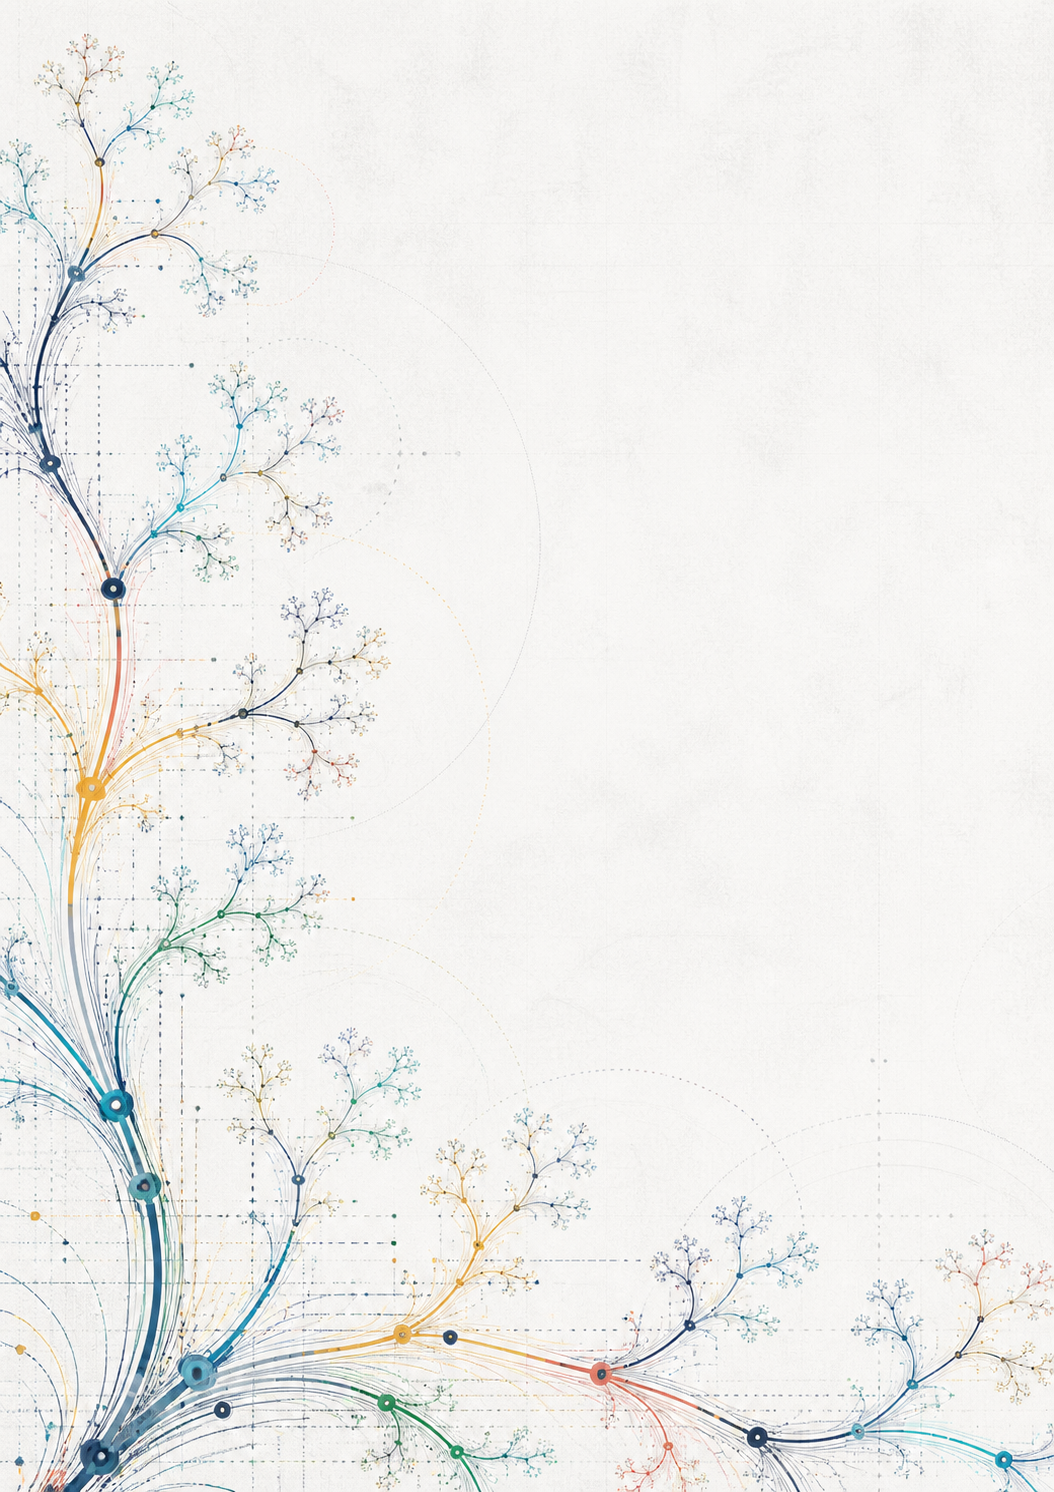
\includegraphics[width=\paperwidth,height=\paperheight]{assets/covers/back-fractal-light.png}}
  \vspace*{1.0in}
  \hspace*{2.25in}\begin{minipage}{3.7in}
  {\sffamily\fontsize{25}{29}\selectfont\bfseries\color{MRInk}Evaluation shapes the system.\par}
  \vspace{0.25in}
  {\sffamily\large\color{MRBlue}This book develops the metric families, their assumptions, their failure modes, and the operating practices that make them useful.\par}
  \vspace{0.35in}
  {\sffamily\normalsize\color{MRInk}Classical IR. RAG grounding. Retriever-generator alignment. Drift. Cost. Judge calibration. Test-set quality. A production dashboard.\par}
  \vspace{0.55in}
  {\sffamily\normalsize\bfseries\color{MRBlue}Madhava Gaikwad\par}
  \end{minipage}
  \vfill
  \ClearShipoutPictureBG
}
